\chapter{\label{cha:title}fuzzing}

In this chapter, we describe a fuzzing algorithm for concurrent programs under weak memory models.

\section{Motivation}

As discussed before, the behaviors of programs under weak memory models are modeled by execution graphs, with nodes representing the events and edges representing the relations. In general, the process of checking such programs is constructing the execution graphs and checking the consistency and validity of the graphs. The search space, or state space, is the set of all possible execution graphs. Due to various combinations of the relations, branches of control flows and loops, he size of the search space can sometimes be quite large or even infinite. For the brevity of discussion, assume the model checker is single-threaded, each time taking one step, either adding a node to the graph or forming a relation between two nodes. In addition, the model checker has some mechanism to ensure the steps taken are valid according to the memory model. Consider the following program: 


\begin{lstlisting}[caption={P1}, label={P1}]
atomic<int> x = {}; // s0

void thread1() {
    x.store(1, relaxed);  // s1 
    x.store(2, relaxed);  // s2 
    x.store(3, relaxed);  // s3 
}
void thread2() {
    int r1 = x.load(relaxed);   // r1
    int r2 = x.load(relaxed);   // r2 
    int r3 = x.load(relaxed);   // r3 
    cout << r1 << r2 << r3 << '\n';
}
\end{lstlisting}

Since all loads and stores are relaxed, the loads will have no synchronization constraints. Each load can have 4 possible stores to read from: s0, s1, s2 and s3. Hence the size of the search space is: $4^3 = 64$. Comparing this with the SC model, if all loads and stores are sc, the total number of executions is $\binom{6}{3} = 20$. 

The probability of finding different executions are not uniform distribution. Some execution graphs are easier to be found, others can have low probability. Consider another example:
\begin{lstlisting}[caption={P2}, label={P2}]
atomic<int> x = {};

void thread1() {
    if(x == 0) {            // a
        if(x == 1)          // b
            if(x == 2) {    // c 
                cout << 'A';
            }
    }
    cout << 'B';
}
void thread2() {
    x++;    // d
    x++;    // e
}
\end{lstlisting}

Suppose the model checker make random decisions uniformly when adding events. The first events in thread 1 and 2 are: x.load() and x++. Thread1 printing 'B' requires that x++ is selected first, with the probability of $\frac{1}{2}$. However, printing 'B' requires a sepecific ordering or selecting events, i.e. {a, d, b, e, c}, with the probability of $\frac{1}{2} \times \frac{1}{2}  \times \frac{1}{2}  \times \frac{1}{2} =  \frac{1}{16}$.


Different orders of adding events and forming relations may result in same executions. Take ~\ref{P1} for example. The model checker can first select r1 first and set its rf as s0, or it can first add s1-3 and then set r1 reading from s0. Both cases are equivalent.

Here is a summary of several challenges or properties of random based model checking for weak memory programs:
\begin{itemize}
    \item The search space of execution graphs are usually large, sometimes infinite.
    \item The probability of finding executions are not uniform. Some infrequent graphs exist.
    \item Different decisions made by the model check may result in same executions.
\end{itemize}

The process of the random-based model checking procedure is similar to the Galton board experiment. Consider the following $n$ level decision tree, from top to bottom, each step has two choices, either going left or right. Each node represents a state and the edges represent the decisions. There are some states that can be reached from multiple paths. Take the middle state in the second level for example, it can be reached by first choosing left then right, or by first choosing right then left. There are also some other states that have more strict requirements on the decision making. For example, the state circled in red requires always select the left choices to reach, with the probability of $\frac{1}{2^n}$. 
\begin{figure}[htbp] % htbp 表示优先放置位置:here, top, bottom, page
    \centering
    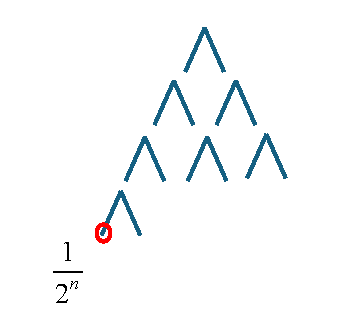
\includegraphics[scale=0.5]{figure/tree.pdf} % 图片文件名和路径  
    \caption{random decision tree} % 图片标题
    \label{tree} % 图片标签,用于交叉引用
\end{figure}


If each time we start from the top and randomly make decisions, those states in the middle will be reached more frequently than those in the corners. However, if we can start from some middle states, it would be easier to reach some corner states, and hence the states reached in the end will be more diverse. This is where our fuzzer come to help. An intuitive description of the fuzzer is: whenever the fuzzer reaches a new state (i.e. finds an interesting execution graph), it mutates one of the decisions made. For the next iteration, the fuzzer replays the decision making until the mutated point, change the decision as mutated, and continues randomly afterwards. As shown in  \ref{tree3} (a), suppose the red path is the previous exploration and the fuzzer mutates the second decision from going right to left (b). Then for the next exploration, it replays until the mutated choice and the probability of reaching the left corner state becomes $\frac{1}{2^{n-2}}$ (c). 

\begin{figure}[htbp] % htbp 表示优先放置位置:here, top, bottom, page
    \centering
    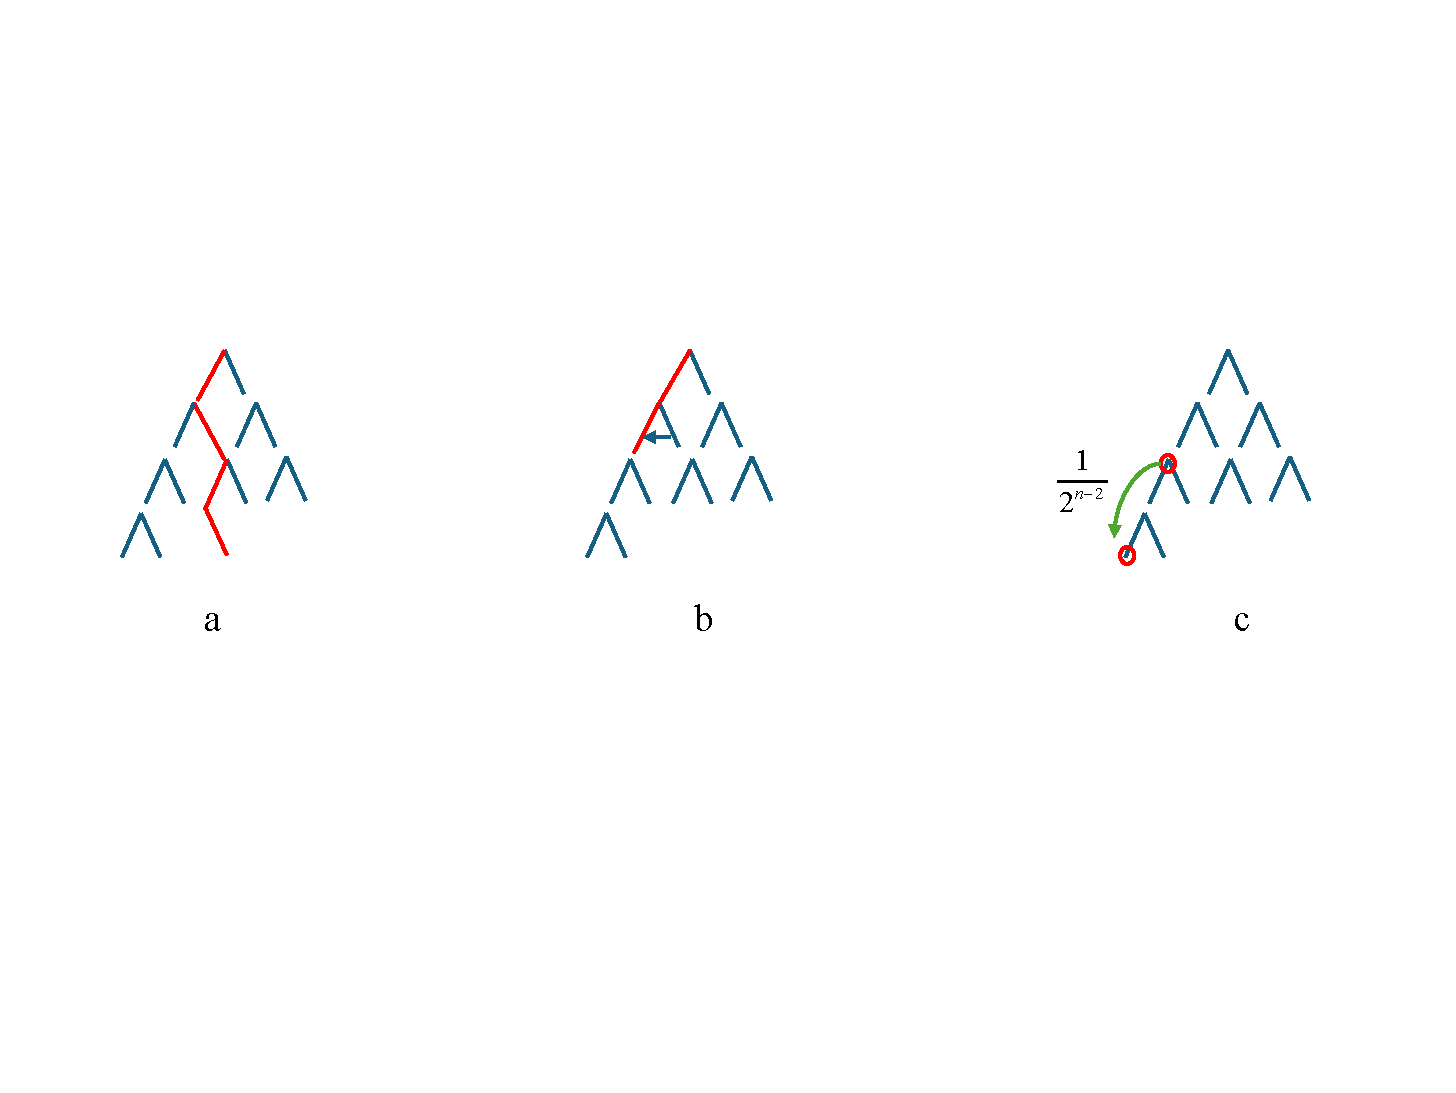
\includegraphics[scale=0.5]{figure/tree3.pdf} % 图片文件名和路径  
    \caption{mutation} % 图片标题
    \label{tree3} % 图片标签,用于交叉引用
\end{figure}


\section{Overview}

\burcu{Could you provide an example of the fuzzing approach on the execution graphs? E.g., Give an example program and a random execution graph of the program. Then, show another execution graph that is obtained by some mutation (e.g., mutates the prev. graph after some prefix) and exposes another behavior of the program.}

This section provides a high-level overview of the fuzzing algorithm. The implementation details and evaluation results will be presented in later chapters.

The fuzzer aims to improve the performance of randomized testing approaches. There are some model checkers, such as C11Tester or GenMC's estimation mode, that uses random-based testing, and some exhaustive model checkers, such as GenMC, that enumerate all possible executions. Exhaustive checkers are useful when the search space is limited, typically when the program under test is not too large. Random-based checking is frequently used for testing large programs. Such a checker usually constructs one execution graph based on random decisions of threads and reads-from relations during each exploration. For the next iteration, it starts over from the beginning and randomly explores again. A problem with this is because it does not keep states among explorations, some repetitive efforts may be taken. Sometimes different random decisions may result in same executions, or some infrequent execution graphs may not be revealed. 

The fuzzer uses partially constructed graphs, represented by "prefix" in the following context, as guidance for further explorations. 
The fuzzer maintains a set of prefixes, initialized empty. At the beginning of each exploration, it pickes a prefix from the set. If there are no existing prefix in the set, the exploration will be random. Otherwise, the model checker will start from the prefix and randomly construct the remaining part of the execution graph. When the exploration is finished, an execution graph will be constructed and the fuzzer will determine whether this execution graph is interesting. The conditions for a graph to be interested could be that it is a new execution graph or it contains some new relations or events. The interested graph will be mutated to generate new prefixes. For example, the fuzzer can change a reads-from relation in that graph and cut out the invalid part after that rf in the graph to get a prefix. The fuzzer may dynamically drop some prefixes based on their ability to find new interesting graphs. Below is a simplified diagram of the fuzzing loop.



\begin{algorithm}
    \caption{Fuzzing algorithm}
    \label{fuzzer}
    \begin{algorithmic}
    \STATE \textbf{Input:} Program $P$ and number of explorations $N$
    \STATE \textbf{Output:} $N$ execution graphs
    
    \STATE prefix\_set $\leftarrow \emptyset$
    \STATE graphs $\leftarrow [ ]$
    
    \FOR{$i \leftarrow 1$ \TO $N$}
        \IF{prefix\_set $\neq \emptyset$}
            \STATE $p \leftarrow$ get\_prefix(prefix\_set)
            \STATE $g \leftarrow $ explore\_from\_prefix($p$)
        \ELSE 
            \STATE $g \leftarrow $ explore\_randomly()
        \ENDIF 
        \IF{is\_interesting(g)}
            \STATE $p' \leftarrow$ mutate(g)
            \STATE prefix\_set $\leftarrow$ prefix\_set $\cup p'$        
        \ENDIF
        \STATE graphs $\leftarrow$ [graphs, g]
    \ENDFOR
    
    \RETURN graphs
    \end{algorithmic}
\end{algorithm}




% \subsection{Threads}





